\chapter{Diseño del experimento}

Utilizando estudios previos de ambas variantes del español pudimos obtener las reglas definidas en el capítulo anterior. Recordemos que estas describen la diferencia entre cada uno de los dos grupos. En este capítulo proponemos realizar un experimento para poder extraer la información fonética de los mismos. La idea será realizar una serie de actividades donde el hablante sea grabado y esas actividades hagan hincapié en estas diferencias descriptas. A continuación vamos a describir el experimento en más detalle.

\section{Elección de las frases}

El acento se potencia cuando se realiza habla espontánea. Utilizando este concepto intentamos que el hablante lo diga de forma lo más natural posible. Es por ello que elegimos como actividad pronunciar frases popularmente conocidas. Si el hablante conoce la frase y la utiliza con frecuencia entonces es más fácil que su pronunciación sea espontánea. Con esta idea vamos a cubrir las reglas 2 al 6. 

Recordemos que en el capítulo anterior la regla 1 nos decía que había una diferencia en la duración de la sílaba previa a la acentuada: para hablantes de Córdoba esta duración es más corta que para hablantes de Buenos Aires. La sílaba acentuada varía según que tipo de palabra se refiere. No es lo mismo utilizar una palabra aguda que una esdrújula en esta regla. Para cubrir esta regla utilizamos un esquema de frases con una estructura fija pero que varía sus palabras según su entonación. Este esquema se llama AMPER \cite{amper} y lo veremos en detalle más adelante.

Entonces los esquemas van a ser: 

\begin{itemize}
  \item \textbf{Frases utilizando esquema AMPER que cubre cada tipo de acentuación:} Estas corresponden a la regla 1 que hace énfasis en la longitud de la sílaba anterior a la acentuada. Utiliza este esquema para cubrir todo tipo de acentuación.
  \item \textbf{Frases comunes que tratan de cubrir la espontaneidad:} Estas frases van a cubrir las reglas 2 a 6. Estas tienen que ver con la duración y la pronunciación de distintos fonemas. Utilizar frases comunes favorece la espontaneidad.
\end{itemize}

A continuación vemos las reglas en sus dos conjuntos.

\subsection{Frases utilizando esquema AMPER}

%AMPER-ARGENTINA: VARIABILIDAD RÍTMICA EN DOS CORPUS 
%Jorge A. Gurlekian LIS - Conicet y UBA jag@fmed.uba.ar 
%Reina Yanagida LIS y Universidad Municipal de Estudios Extranjeros de Kobe, Japón reinay@hotmail.co.jp 
%Mónica Noemí Trípodi LIS – UBA monica906@hotmail.com 
%Guillermo Toledo Conicet y Universidad Laval, Canadá guillermo.toledo@sympatico.ca 

Utilizamos este esquema para analizar todas las variantes posibles de la regla 1. Recordemos que esa regla nos dice que hay que estirar la sílaba anterior a la acentuada. Esta regla define comúnmente la tonada cordobeza y puede aparecer de varias formas según su acentuación. 

Para tomar este esquema nos basamos en el trabajo de variabilidad rítmica en dos corpus \cite{amper} donde utilizan un esquema similar. Este trabajo estudió los acentos del español argentino utilizando todas sus combinaciones. En nuestro trabajo tenemos un problema similar por ello lo tomamos como referencia.

Para el esquema AMPER se fija un patrón de estructura de frases y se va cambiando las palabras que utiliza. 
El esquema AMPER utilizado en este trabajo es: 
\begin{center}
\textit{Sujeto+`` salió ’’+Adjetivo} 
\end{center}

\begin{itemize}
	\item Objeto puede ser \textit{``El canapé’’, ``El repollo’’, ``El espárrago’’}.
	\item Adjetivo puede ser \textit{``espectacular’’, ``delicioso’’, ``riquísimo’’}.
\end{itemize}

Utilizamos estas palabras ya que cubren los tres tipos de acentuación, o sea pasa por aguda, grave y esdrújula. 

Por ejemplo: \textit{``El canapé salió delicioso’’}. Canapé tiene acento en la última sílaba, es una palabra aguda, mientras que delicioso es grave. En este ejemplo podemos analizar la sílaba anterior a la acentuada de estos dos grupos. Armamos las combinaciones para obtener muchas variantes de dónde se encuentra el acento. De esta forma estudiamos en detalle la regla 1. Todas las combinaciones se pueden ver en el tabla \ref{fig21table}.

%\begin{figure}[h!]
%    \centerline{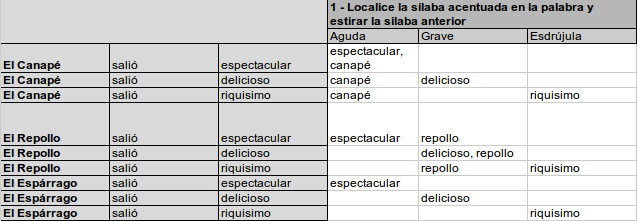
\includegraphics[width=1\textwidth]{reglas_AMPER} }
%    \caption{Frases AMPER}
%    \label{fig21}
%\end{figure}

\scriptsize
\begin{longtable}{| p{0.15\textwidth} | p{0.08\textwidth} | p{0.15\textwidth} || p{0.15\textwidth} | p{0.15\textwidth} | p{0.15\textwidth} |} 
	\hline
	\multicolumn{6}{| p{0.9\textwidth} |} {\textbf{1 - Localice la sílaba acentuada en la palabra y estirar la sílaba anterior}} \\ \hline
	\multicolumn{3}{| p{0.45\textwidth} ||}{Frase} & \textbf{Aguda} & \textbf{Grave} & \textbf{Esdrújula} \\ \hline 
	\textit{El canapé} & \textit{salió} & \textit{espectacular} & espectacular, canapé & & \\ \hline
	\textit{El canapé} & \textit{salió} & \textit{delicioso} & canapé & delicioso & \\ \hline
	\textit{El canapé} & \textit{salió} & \textit{riquísimo} & canapé & & riquísimo \\ \hline
	\textit{El repollo} & \textit{salió} & \textit{espectacular} & espectacular & repollo & \\ \hline
	\textit{El repollo} & \textit{salió} & \textit{delicioso} &  & repollo, delicioso & \\ \hline	
	\textit{El repollo} & \textit{salió} & \textit{riquísimo} & & repollo & riquísimo \\ \hline
	\textit{El espárrago} & \textit{salió} & \textit{espectacular} & espectacular & & \\ \hline
	\textit{El espárrago} & \textit{salió} & \textit{delicioso} & & delicioso & \\ \hline
	\textit{El espárrago} & \textit{salió} & \textit{riquísimo} & & & riquísimo \\ \hline	
		
	\caption{Frases AMPER} 
	\label{fig21table}
\end{longtable}

\normalsize
\subsection{Frases comunes}

Como afirmamos antes, se utilizaron frases comunes para poder obtener los acentos de cada grupo de forma natural. Se pensó que si se graba una frase popular, el hablante al estar acostumbrado a decirla no iba a poder evitar impregnarle su acento. Todas las frases conocidas utilizadas se pueden ver en la tabla \ref{fig22tabla}.

%\begin{figure}[h!]
%    \centerline{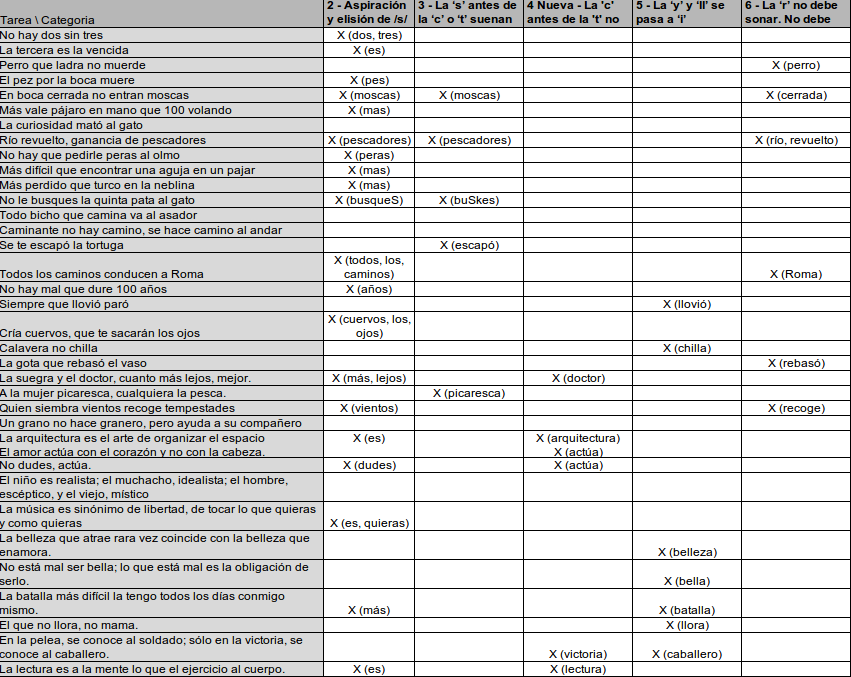
\includegraphics[width=1\textwidth]{frases_inf} }
%    \caption{Frases conocidas}
%    \label{fig22}
%\end{figure}

\newgeometry{margin=2cm} 
\begin{landscape}
\scriptsize
\begin{longtable}{| p{0.5\textwidth} || p{0.15\textwidth} | p{0.15\textwidth} | p{0.15\textwidth} | p{0.15\textwidth}| p{0.15\textwidth} | } 
	\hline
	\textbf{Frase} & \textbf{2 - Aspiración y elisión de /s/} & \textbf{3 - La 's' antes de la 'c' o 't' no suenan} & \textbf{4 - La 'c' antes de la 't' no suenan}& \textbf{5 - La 'y' y 'll' se pasa a 'i'} & \textbf{6 - La 'r' no debe sonar} \\ \hline	
	
	
	'No hay dos sin tres' & dos, tres & & & & \\ \hline
	'Más difícil que encontrar una aguja en un pajar' & más &&&& \\ \hline
	'Más perdido que turco en la neblina' & más &&&&  \\ \hline
	'No le busques la quinta pata al gato' & busques & busques &&&  \\ \hline
%	'Todo bicho que camina va al asador' &  \\ \hline
%	'Caminante no hay camino se hace camino al andar' &  \\ \hline
	'Se te escapó la tortuga' && escapó &&&  \\ \hline
	'Todos los caminos conducen a Roma' & todos, los, caminos &&&&  \\ \hline
	'No hay mal que dure cien anos' & años &&&& \\ \hline
	'Siempre que llovió paro' &&&& llovió & \\ \hline
	'Cría cuervos que te sacaran los ojos' & cuervos, los, ojos &&&&  \\ \hline
	'La tercera es la vencida' & es &&&& \\ \hline
	'Calavera no chilla' &&&& chilla &  \\ \hline
	'La gota que rebalsó el vaso' &&&&& rebasó \\ \hline
	'La suegra y el doctor cuanto más lejos mejor' & más, lejos & doctor&&& \\ \hline
	'A la mujer picaresca cualquiera la pesca' && picaresca &&&  \\ \hline
	'Quien siembra vientos recoge tempestades' & vientos &&&& recoge  \\ \hline
%	'Un grano no hace granero pero ayuda a su compañero' & \\ \hline
	'La arquitectura es el arte de organizar el espacio' & es && arquitectura && \\ \hline
	'El amor actúa con el corazón y no con la cabeza' &&& actúa&& \\ \hline
	'No dudes actúa' &&& actúa&&  \\ \hline
%	'El niño es realista; el muchacho, idealista; el hombre, escéptico, y el viejo místico' &  \\ \hline
	'Perro que ladra no muerde' &&&&& perro \\ \hline
	'La musica es sinónimo de libertad, de tocar lo que quieras y como quieras' & es, quieras &&&& \\ \hline
	'La belleza que atrae rara vez coincide con la belleza que enamora' &&&& belleza & \\ \hline
	'No esta mal ser bella lo que esta mal es la obligación de serlo' &&&& bella & \\ \hline
	'La batalla más difícil la tengo todos los días conmigo mismo' & más &&& batalla & \\ \hline
	'El que no llora no mama' &&&& llora & \\ \hline
	'En la pelea se conoce al soldado solo en la victoria se conoce al caballero' &&& victoria & caballero &\\ \hline
	'La lectura es a la mente lo que el ejercicio al cuerpo' & es && lectura &&  \\ \hline
	'El pez por la boca muere' & pez &&&& \\ \hline
	'En boca cerrada no entran moscas' & moscas & moscas &&& cerrada  \\ \hline
	'Más vale pájaro en mano que cien volando' & más &&&& \\ \hline
%	'La curiosidad mató al gato' &  \\ \hline
	'Río revuelto ganancia de pescadores' & pescadores & pescadores &&& río, revuelto  \\ \hline
	'No hay que pedirle peras al olmo' & peras &&&& \\ \hline
	
	\caption{Frases conocidas} 
	\label{fig22tabla}
\end{longtable}
\end{landscape}
\restoregeometry

\normalsize

Algo interesante es que una misma frase puede extraer atributos para varias reglas. Por ejemplo: la frase \textit{`En la pelea se conoce al soldado, sólo en la victoria se conoce al caballero’} extrae atributos para las reglas 4 y 5. La palabra \textit{`victoria’} cubre la regla 4 que nos propone medir la duración de la \textit{/c/} antes de la \textit{/t/}. Sucede igual con la palabra \textit{`caballero’} para la regla 5: el fonema \textit{/ll/} se pasa a \textit{/i/} cambiando su duración y sonido. De esta forma cada frase tiene el mayor cubrimiento posible. En la Tabla \ref{fig22tabla} podemos ver que la cantidad de frases utilizadas con respecto a sus reglas es despareja. Hay más frases para la regla 2 que para las demás. Más adelante veremos como impacta esto en las frases que vamos a pedir grabar.

\subsubsection{Orden de las frases}

Ya definimos cuales van a ser las frases, ahora debemos definir qué frases y en qué orden se deben decir durante el experimento. Sucede que el orden que utilicemos va a ser crucial para obtener muestras: no es lo mismo empezar por una frase que solo cubre una sola regla que varias. Si elegimos primero las frases que cubren varias reglas a la vez, en un solo audio podremos obtener más cubrimiento de reglas. 

¿Porqué quisiéramos cubrir mas reglas en una misma frase? Más adelante veremos que una frase grabada que cubre una regla aportará información sobre el hablante de esa regla en particular. Si una frase cubre varias reglas estaríamos obteniendo más información y solo con una grabación. Por eso es importante maximizar el cubrimiento de las frases.  

El orden de las frases sigue el siguiente algoritmo:

\lstset{ %
language=C++,                % choose the language of the code
basicstyle=\footnotesize,       % the size of the fonts that are used for the code
numbers=left,                   % where to put the line-numbers
numberstyle=\footnotesize,      % the size of the fonts that are used for the line-numbers
stepnumber=1,                   % the step between two line-numbers. If it is 1 each line will be numbered
numbersep=5pt,                  % how far the line-numbers are from the code
backgroundcolor=\color{white},  % choose the background color. You must add \usepackage{color}
showspaces=false,               % show spaces adding particular underscores
showstringspaces=false,         % underline spaces within strings
showtabs=false,                 % show tabs within strings adding particular underscores
frame=single,           % adds a frame around the code
tabsize=2,          % sets default tabsize to 2 spaces
captionpos=b,           % sets the caption-position to bottom
breaklines=true,        % sets automatic line breaking
breakatwhitespace=false,    % sets if automatic breaks should only happen at whitespace
escapeinside={\%*}{*)},          % if you want to add a comment within your code
morekeywords={GeneradorDeTest, GenradorDeTrazas, checkBalance, Input, Output, Repetir, veces, Si, agregar, Recorrer, Devolver, y, no, esta, en, Mientras},
}
\begin{lstlisting}
    OrdenDeFrasesConocidas:
    Input: Frases
    Output: listaFrases 
    listaFrases = {}
    DicPct <- Diccionario de porcentajes de cada regla
    Mientras Frases != {}:
    	regla <- ObtenerReglaConMejorPorcentaje(DicPct)
    	frase <- Frases.ObtenerLaMasPonderada(regla)
    	listaFrases.agregar(frase)
    	RecalcularPorcentajes(DicPct)
    Devolver listaFrases
\end{lstlisting}

La idea del algoritmo es la siguiente: vamos a utilizar un contador que nos va a decir cuántas muestras tenemos por cada regla. En cada paso vamos a ver ese contador y vamos a elegir la próxima frase teniéndolo en cuenta. Esta elección la lleva a cabo la función \textit{ObtenerLaMasPonderada}. Esta se encarga de elegir la frase que haga referencia a la regla menos grabada y además que represente a más de una regla. De esa forma intentamos obtener la mayor cantidad de información posible con pocas grabaciones y ponderamos las frases que referencien a más reglas. 

Esta idea es importante ya que llevamos al máximo la cantidad de información en cada frase y al hablante le hacemos perder menos tiempo realizando el experimento. Esto se puede ver en la Figura \ref{figFracesTraza} que representa el porcentaje de frases completadas mientras se va aumentando la cantidad de grabaciones. Teniendo en cuenta este algoritmo podemos notar que aproximadamente a partir de 10 grabaciones ya tenemos un buen porcentaje de cubrimiento de alrededor del 40\% en todas las reglas.

%\begin{figure}[h!]
%    \centerline{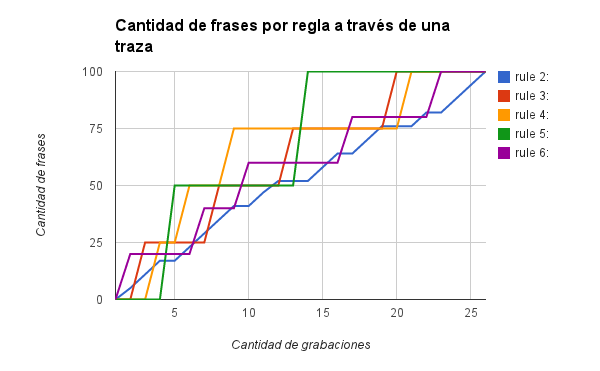
\includegraphics[width=0.9\textwidth]{cant_frases_traza_inf} }
    %\caption{Cantidad de frases por traza}
    %\label{figFracesTraza}
%\end{figure}

\begin{figure}[H]
	\centering
	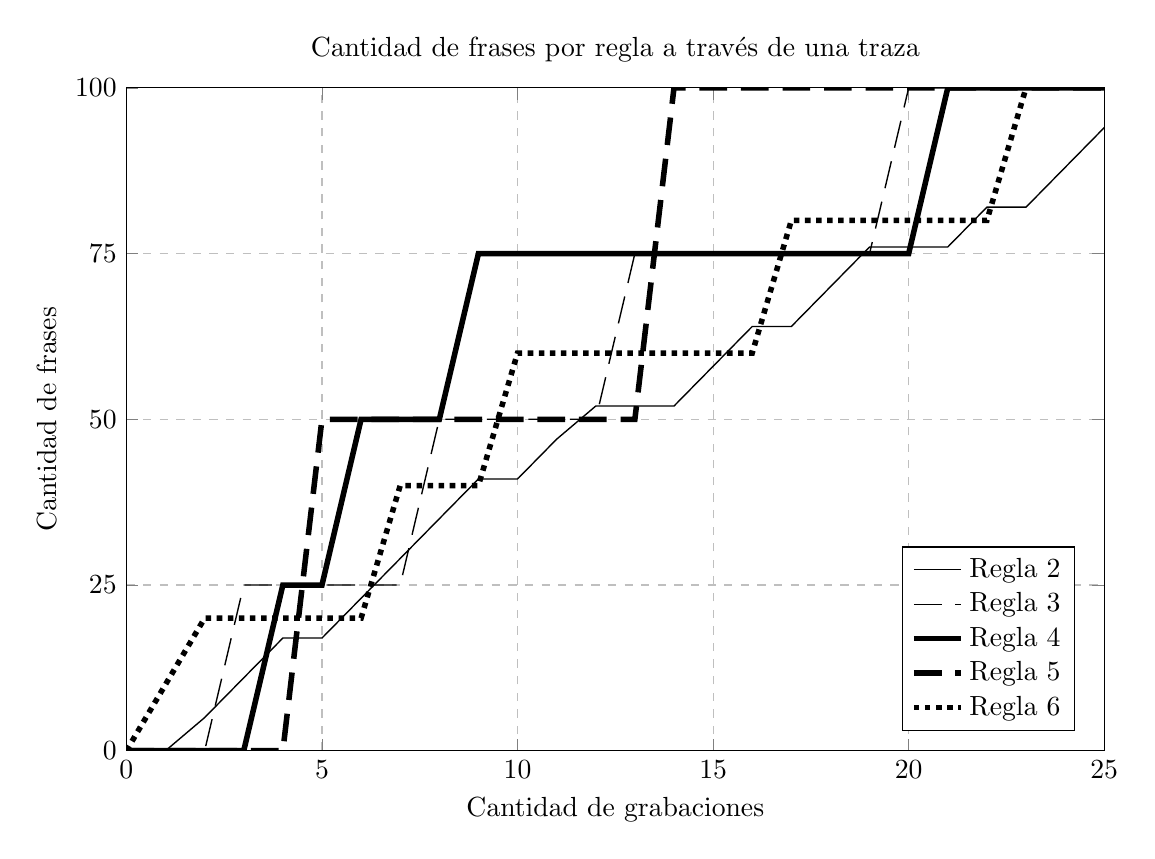
\begin{tikzpicture}
	\begin{axis}[
	width=14cm,
	height=10cm,
	title={Cantidad de frases por regla a través de una traza},
	xlabel={Cantidad de grabaciones},
	ylabel={Cantidad de frases},
	xmin=0, xmax=25,
	ymin=0, ymax=100,
	xtick={0,5,10,15,20,25,30},
	ytick={0, 25, 50, 75, 100},
	legend pos=south east,
	ymajorgrids=true,
	xmajorgrids=true,
	grid style=dashed
	] 
	
	\addplot [mark=times*, line width=0.5pt]
	coordinates {
  		(0,0)(1, 0)(2, 5)(3, 11)(4, 17)(5, 17)(6, 23)(7, 29)(8, 35)(9, 41)(10, 41)(11, 47)(12, 52)(13, 52)(14, 52)(15,58)(16, 64)(17, 64)(18, 70)(19, 76)(20, 76)(21, 76)(22, 82)(23, 82)(24, 88)(25, 94)(26, 100)
	};\addlegendentry{Regla 2};
	
	\addplot [mark=times*, dash pattern=on 10pt off 5pt, line width=0.5pt]
	coordinates {
		(0,0)(1,0)(2,0)(3,25)(4,25)(5,25)(6,25)(7,25)(8,50)(9,50)(10,50)(11,50)(12,50)(13,75)(14,75)(15,75)(16,75)(17,75)(18,75)(19,75)(20,100)(21,100)(22,100)(23,100)(24,100)(25,100)(26,100)
	};\addlegendentry{Regla 3};
	
	\addplot [mark=times*, line width=2pt] 
	coordinates {
		(0,0)(1, 0)(2, 0)(3, 0)(4, 25)(5, 25)(6, 50)(7, 50)(8, 50)(9, 75)(10, 75)(11, 75)(12, 75)(13, 75)(14, 75)(15,75)(16, 75)(17, 75)(18, 75)(19, 75)(20, 75)(21, 100)(22, 100)(23, 100)(24,100)(25,100)(26, 100)
	};\addlegendentry{Regla 4};
	
	\addplot [mark=times*, dash pattern=on 10pt off 5pt, line width=2pt]
	coordinates {
		(0,0)(4,0)(5,50)(13,50)(14,100)(26,100) 
	};\addlegendentry{Regla 5};
	
	\addplot [mark=times*, dotted, line width=2pt] 
	coordinates {
		(0,0)(2,20)(6,20)(7,40)(9,40)(10,60)(16,60)(17,80)(22,80)(23,100) 
	};\addlegendentry{Regla 6};
		
		
%%		Tarea	rule 2:	rule 3:	rule 4:	rule 5:	rule 6:
%		1	0	0	0	0	0
%		2	5	0	0	0	20
%		3	11	25	0	0	20
%		4	17	25	25	0	20
%		5	17	25	25	50	20
%		6	23	25	50	50	20
%		7	29	25	50	50	40
%		8	35	50	50	50	40
%		9	41	50	75	50	40
%		10	41	50	75	50	60
%		11	47	50	75	50	60
%		12	52	50	75	50	60
%		13	52	75	75	50	60
%		14	52	75	75	100	60
%		15	58	75	75	100	60
%		16	64	75	75	100	60
%		17	64	75	75	100	80
%		18	70	75	75	100	80
%		19	76	75	75	100	80
%		20	76	100	75	100	80
%		21	76	100	100	100	80
%		22	82	100	100	100	80
%		23	82	100	100	100	100
%		24	88	100	100	100	100
%		25	94	100	100	100	100
%		26	100	100	100	100	100
		
	\end{axis}
	\end{tikzpicture}
    \caption{Cantidad de frases por traza}
    \label{figFracesTraza}
\end{figure}


\subsection{Combinando los dos tipos de frases utilizando trazas}

Definimos ambos tipos de frases a grabar. Ahora debemos definir como vamos a ir intercalando cada tipo en el experimento, para ello definimos traza. Una traza es una lista de las frases que va a grabar un hablante en el experimento. Esta va a estar compuesta entre 1 ó 3 frases comunes extraídas del orden definido en \textit{OrdenDeFrasesConocidas}, y luego una frase del esquema de AMPER. Tanto la cantidad de frases comunes como la elección de la frase AMPER se realiza al azar. Este patrón se repite sucesivamente hasta completar todas las frases. La idea es no cansar al hablante con frases repetitivas y evitar que sepa de antemano qué frase va a tener que grabar. 

Al empezar el experimento, al hablante se le dará una traza que grabará sucesivamente en ese orden. Elegimos tener precalculadas las trazas para evitar cálculos costosos a la hora de empezar el experimento. Si no se precalcularan las trazas, deberíamos realizar los cálculos cada vez que empieza el experimento y podríamos retrasar la grabación del hablante. Es por eso que guardamos 10.000 trazas generadas. 

La mínima cantidad de grabaciones que puede realizar un hablante son 5 grabaciones. Luego se le pregunta si quiere continuar grabando. Si acepta, se le agregan otras 5 grabaciones así sucesivamente hasta llegar al total de frases a grabar. Elegimos grabar cada 5 grabaciones para que el hablante aporte el tiempo que tenga disponible y no obligarlo a grabar todas las frases. Aunque no grabe la totalidad de frases, las muestras van a servir en el experimento.

A continuación veremos como implementamos el sistema de grabación para soportar este experimento.